% Document class, paper size, base font size
\documentclass[a4paper, 12pt]{article}

% Encoding
\usepackage[utf8]{inputenc}
\usepackage[T1]{fontenc}

% Prevent indentation of beginning of paragraphs
\setlength{\parindent}{0em}

% Space between paragraphs
\parskip 0.5em

% include PDFs
\usepackage{pdfpages}

% Title, authors and date
\title{Exercise 5: UML}
\author{
    Kendra Birringer (1229372)\\
    Nader Cacace (1208115)\\
    Steffen Hanzlik (1207417)\\
    Marco Peluso (1228849)\\
    Svetozar Stojanovic (1262287)\\
    \\
    Frankfurt University of Applied Sciences
}
\date{November 16, 2019}


% Begin actual document
\begin{document}

\maketitle
\newpage
\tableofcontents

\newpage
\section{Redesign Diagram Figure 18.1 (from UML Standard 2.5.1 Specification\cite{uml251specpdf}}
\begin{center}
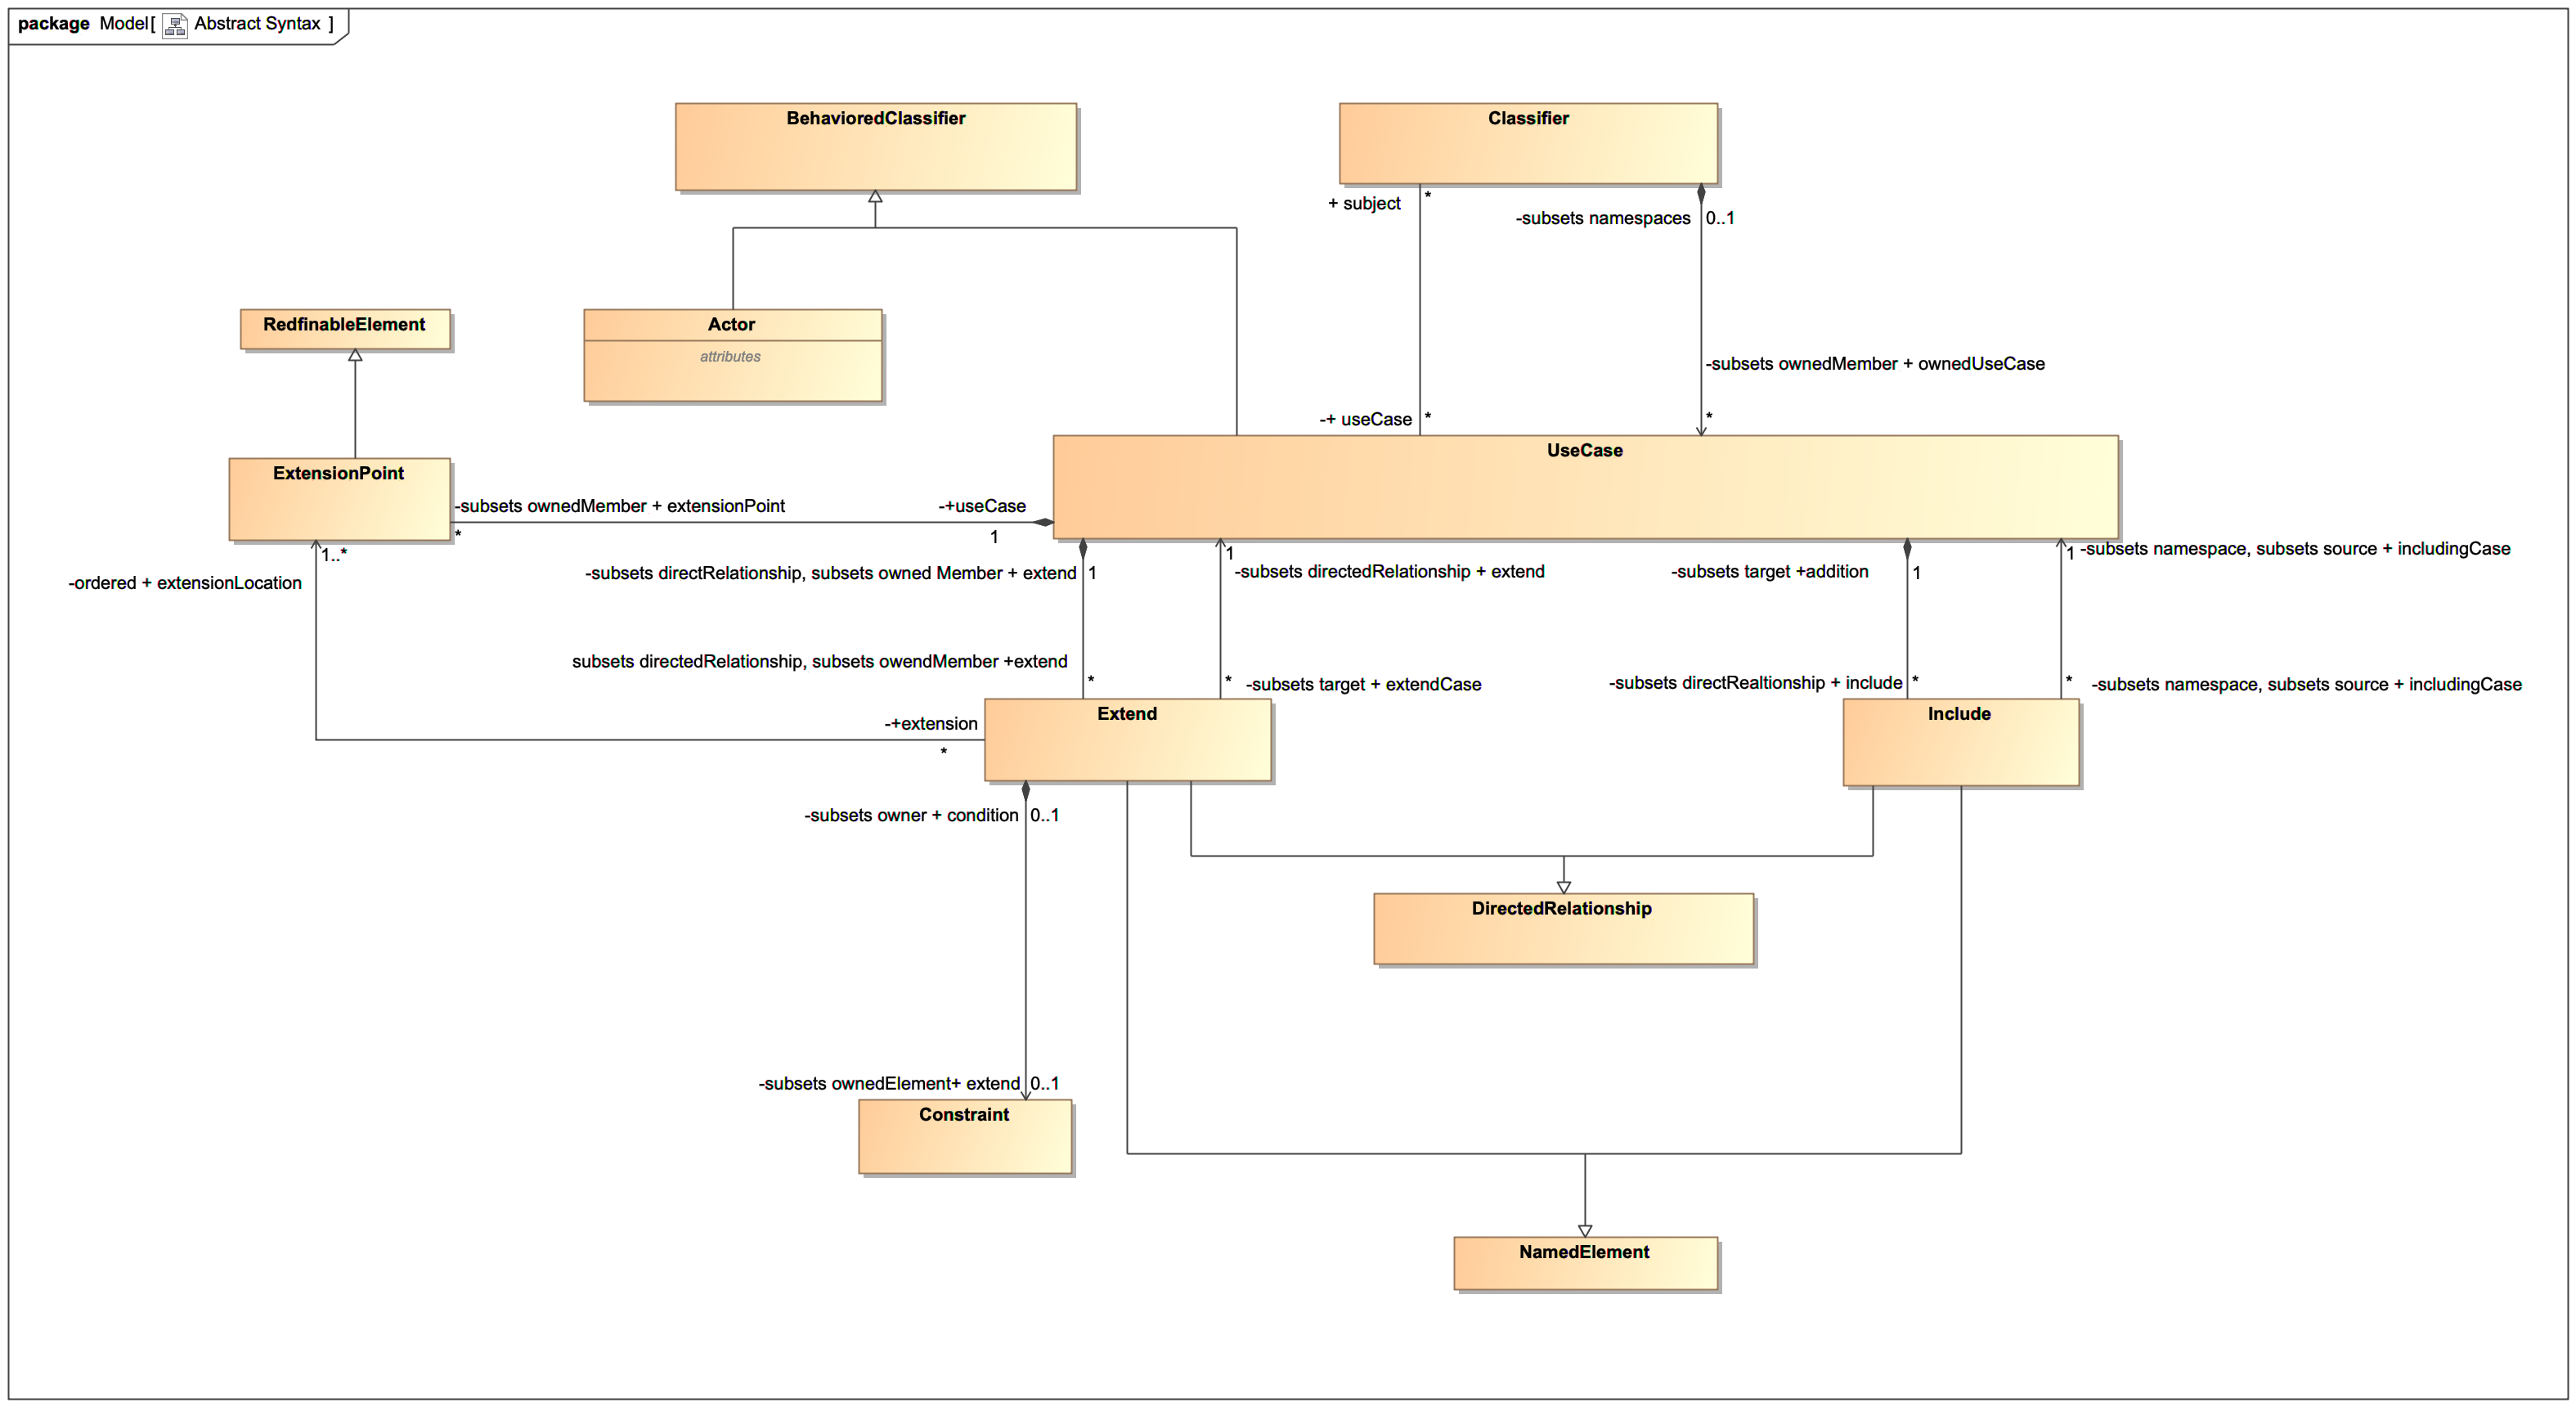
\includegraphics[scale=0.4, angle=90, origin=c]{01-abstract-syntax.png}
\end{center}

\section{Use Case: Customer registration and Administration}
\begin{center}
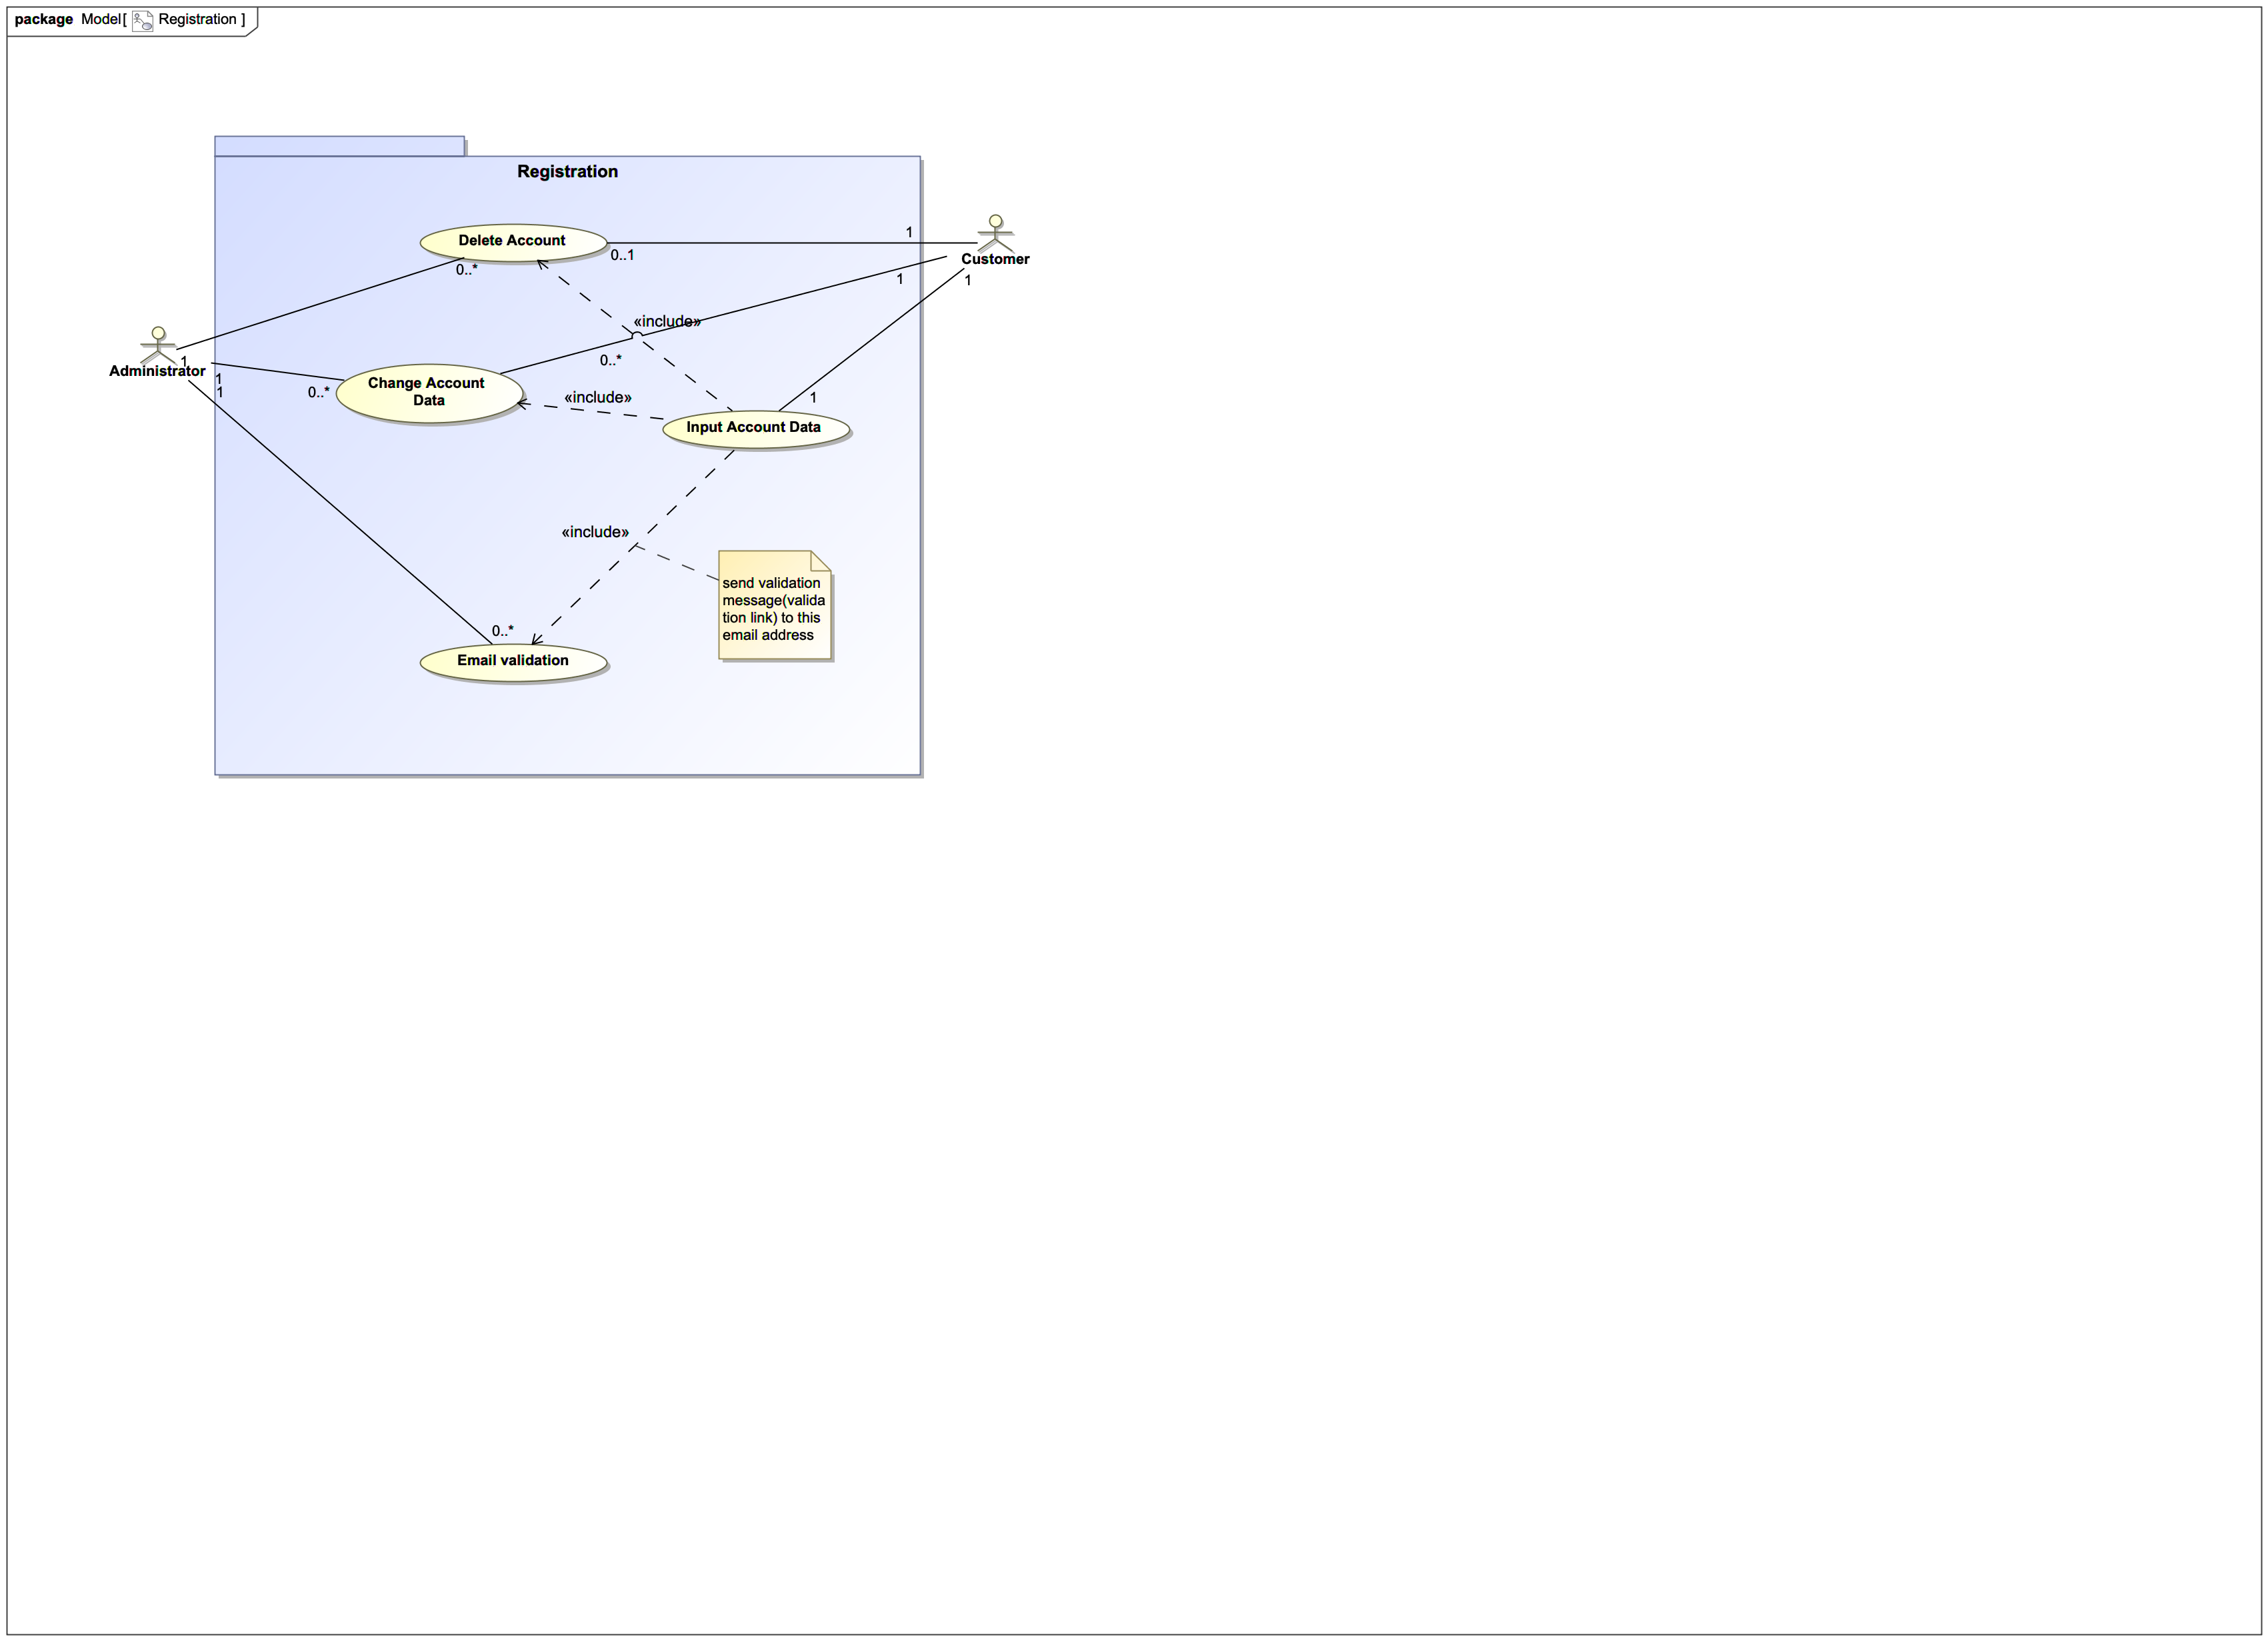
\includegraphics[scale=0.5]{02-e-bike-rental-service-variant-1-01.png}
\end{center}

\section{Use Case: Payment by an External Bank}
\begin{center}
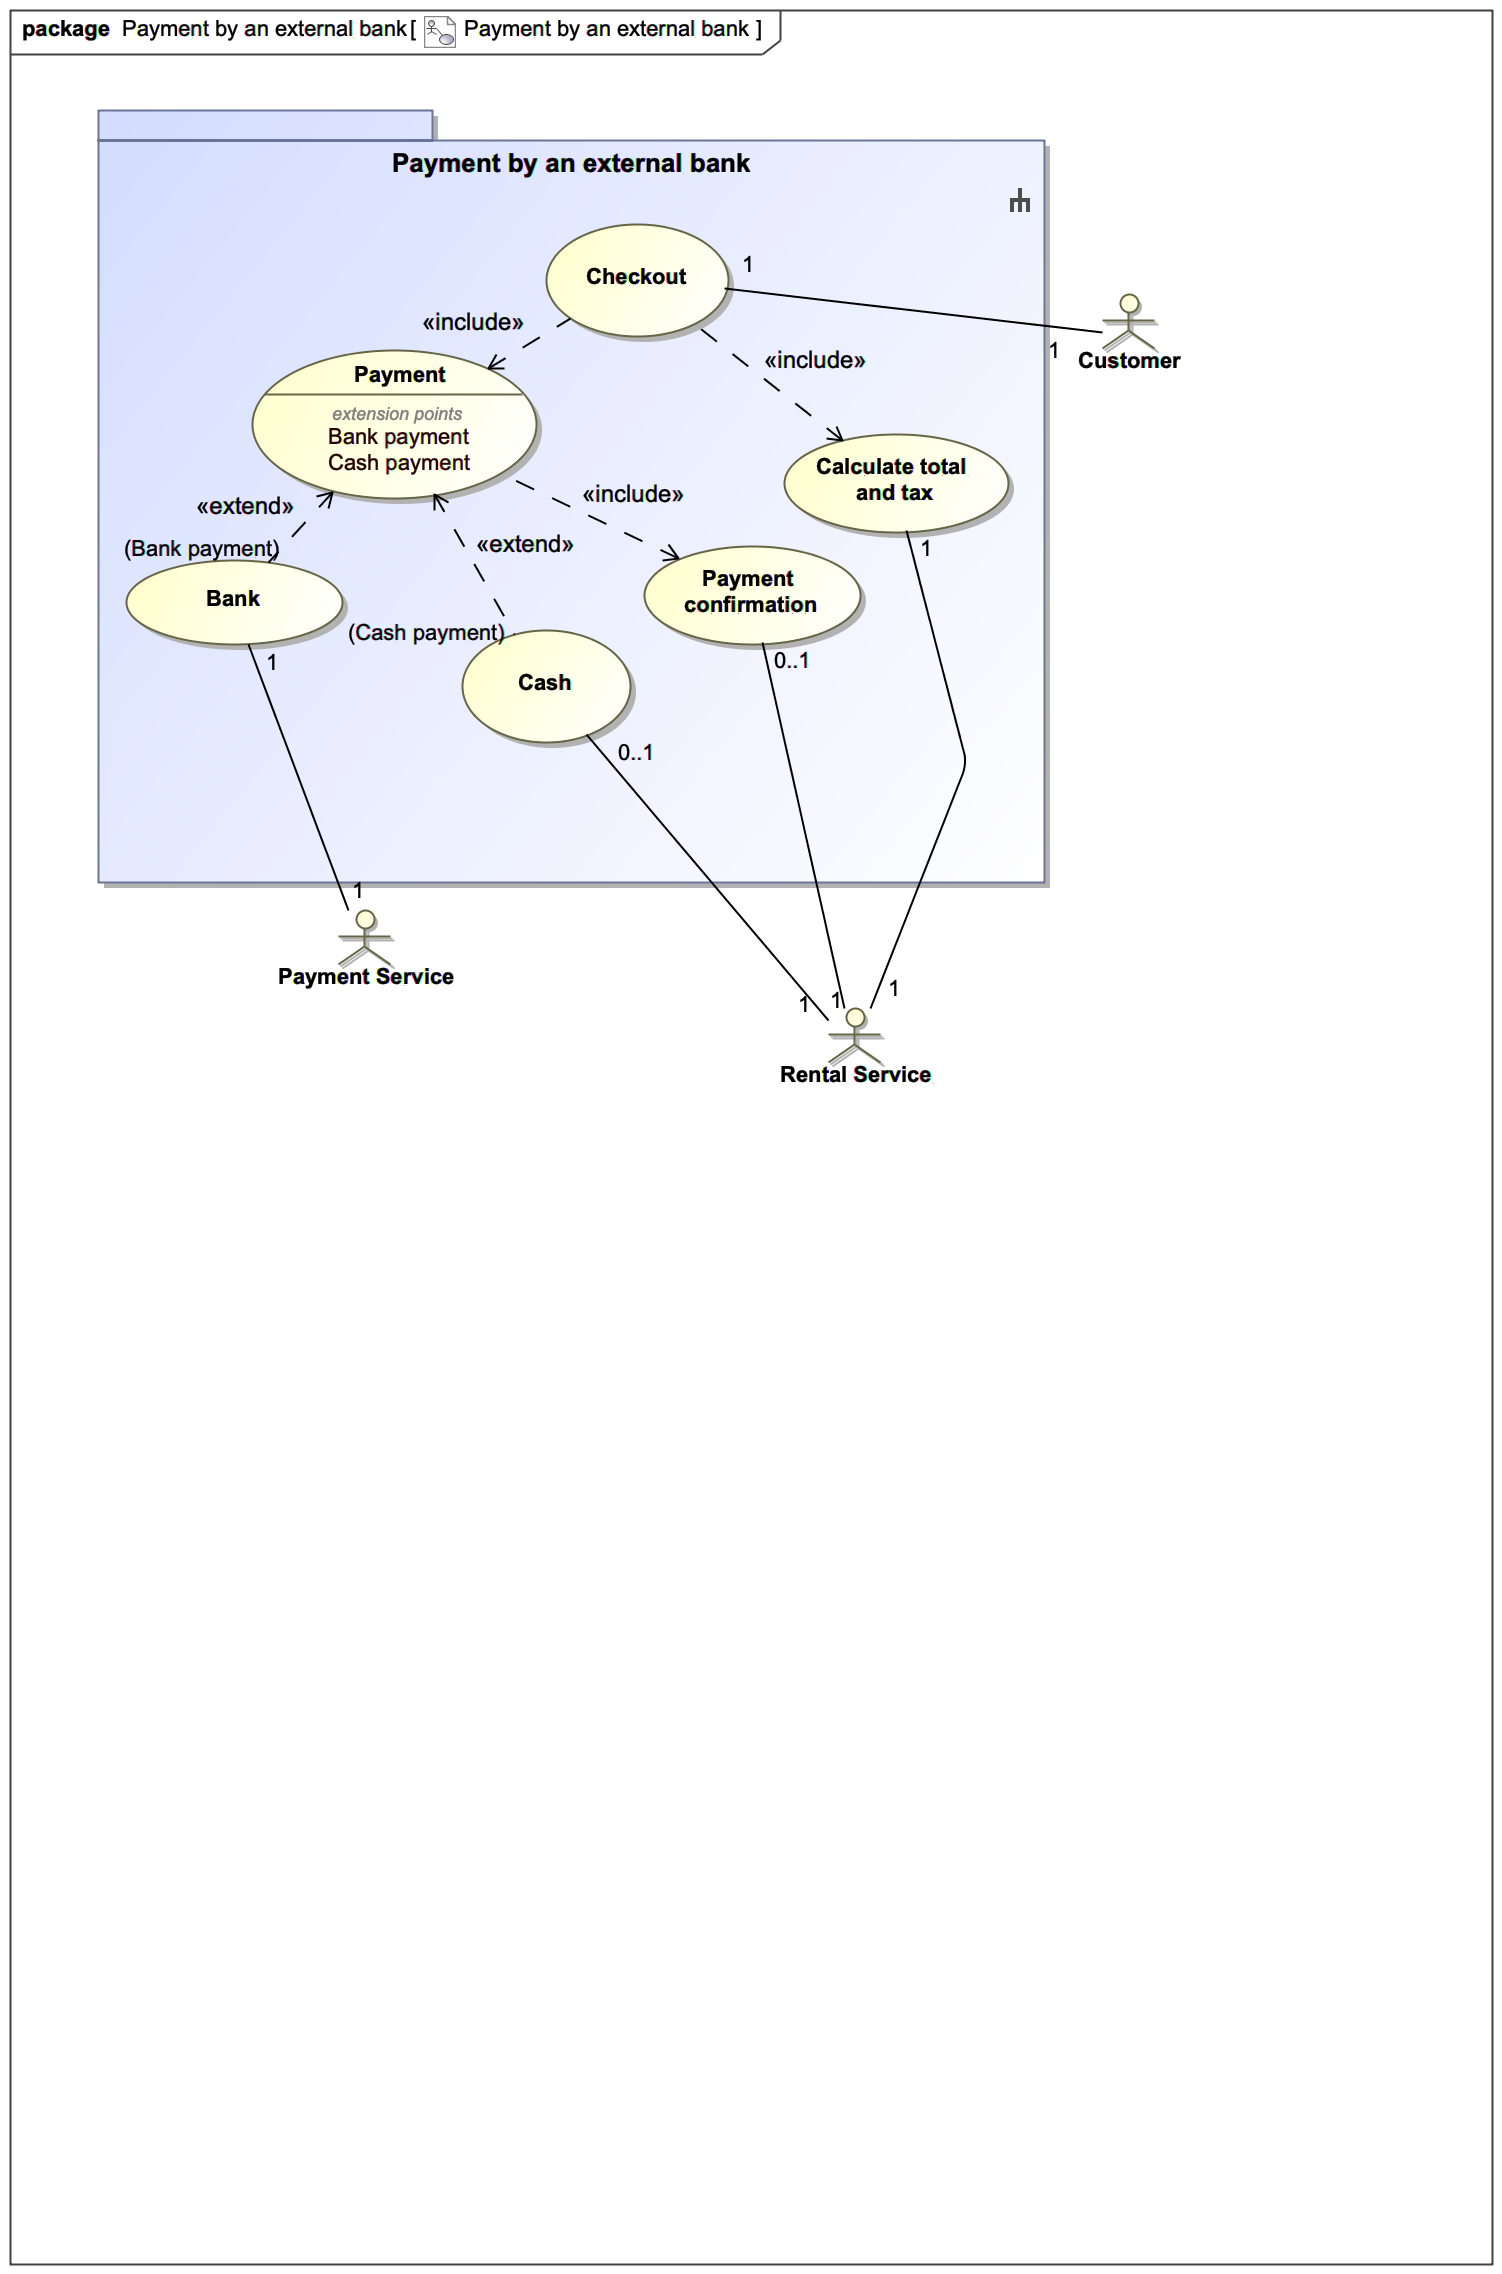
\includegraphics[scale=0.5]{02-e-bike-rental-service-variant-1-02.png}
\end{center}

\section{Use Case: Check-in/-out for Bicycle Rent}
\begin{center}
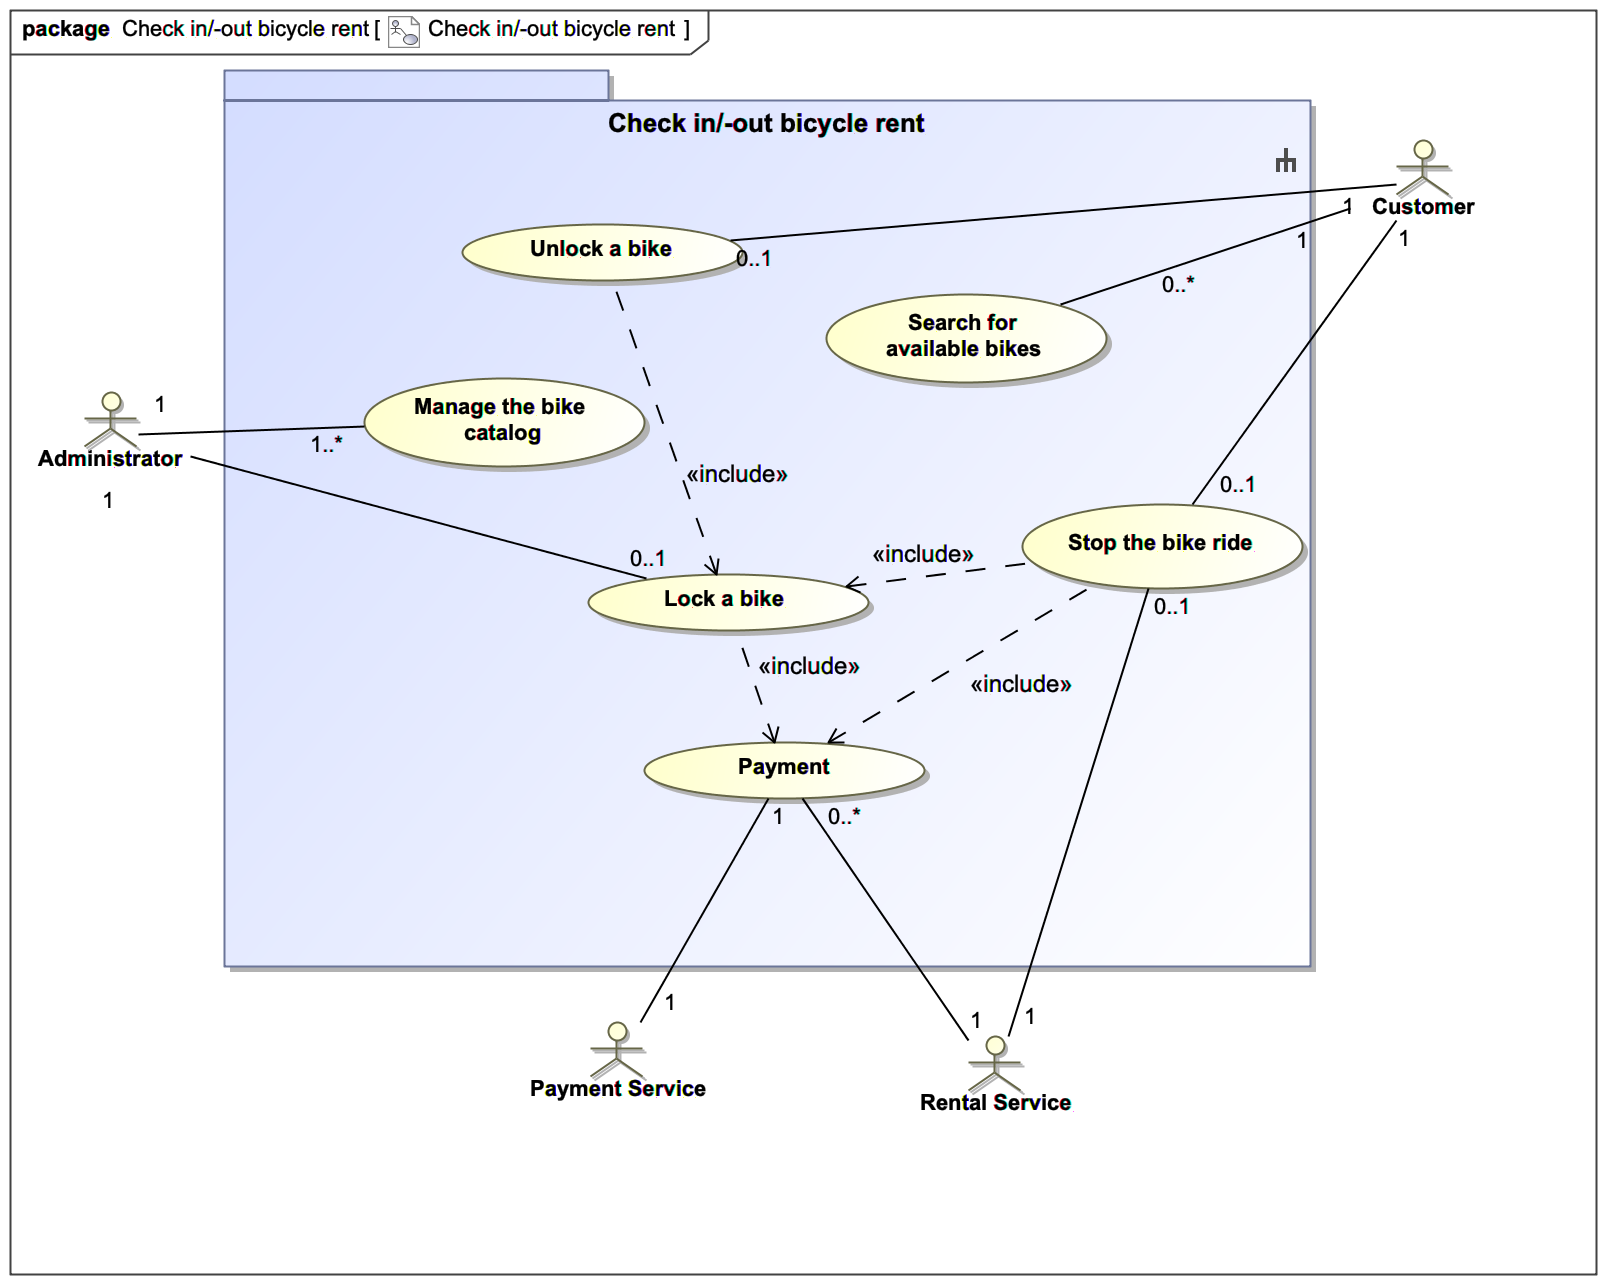
\includegraphics[scale=0.5]{02-e-bike-rental-service-variant-1-03.png}
\end{center}

\section{Use Cases (Variant 2: Combined)}
\begin{center}
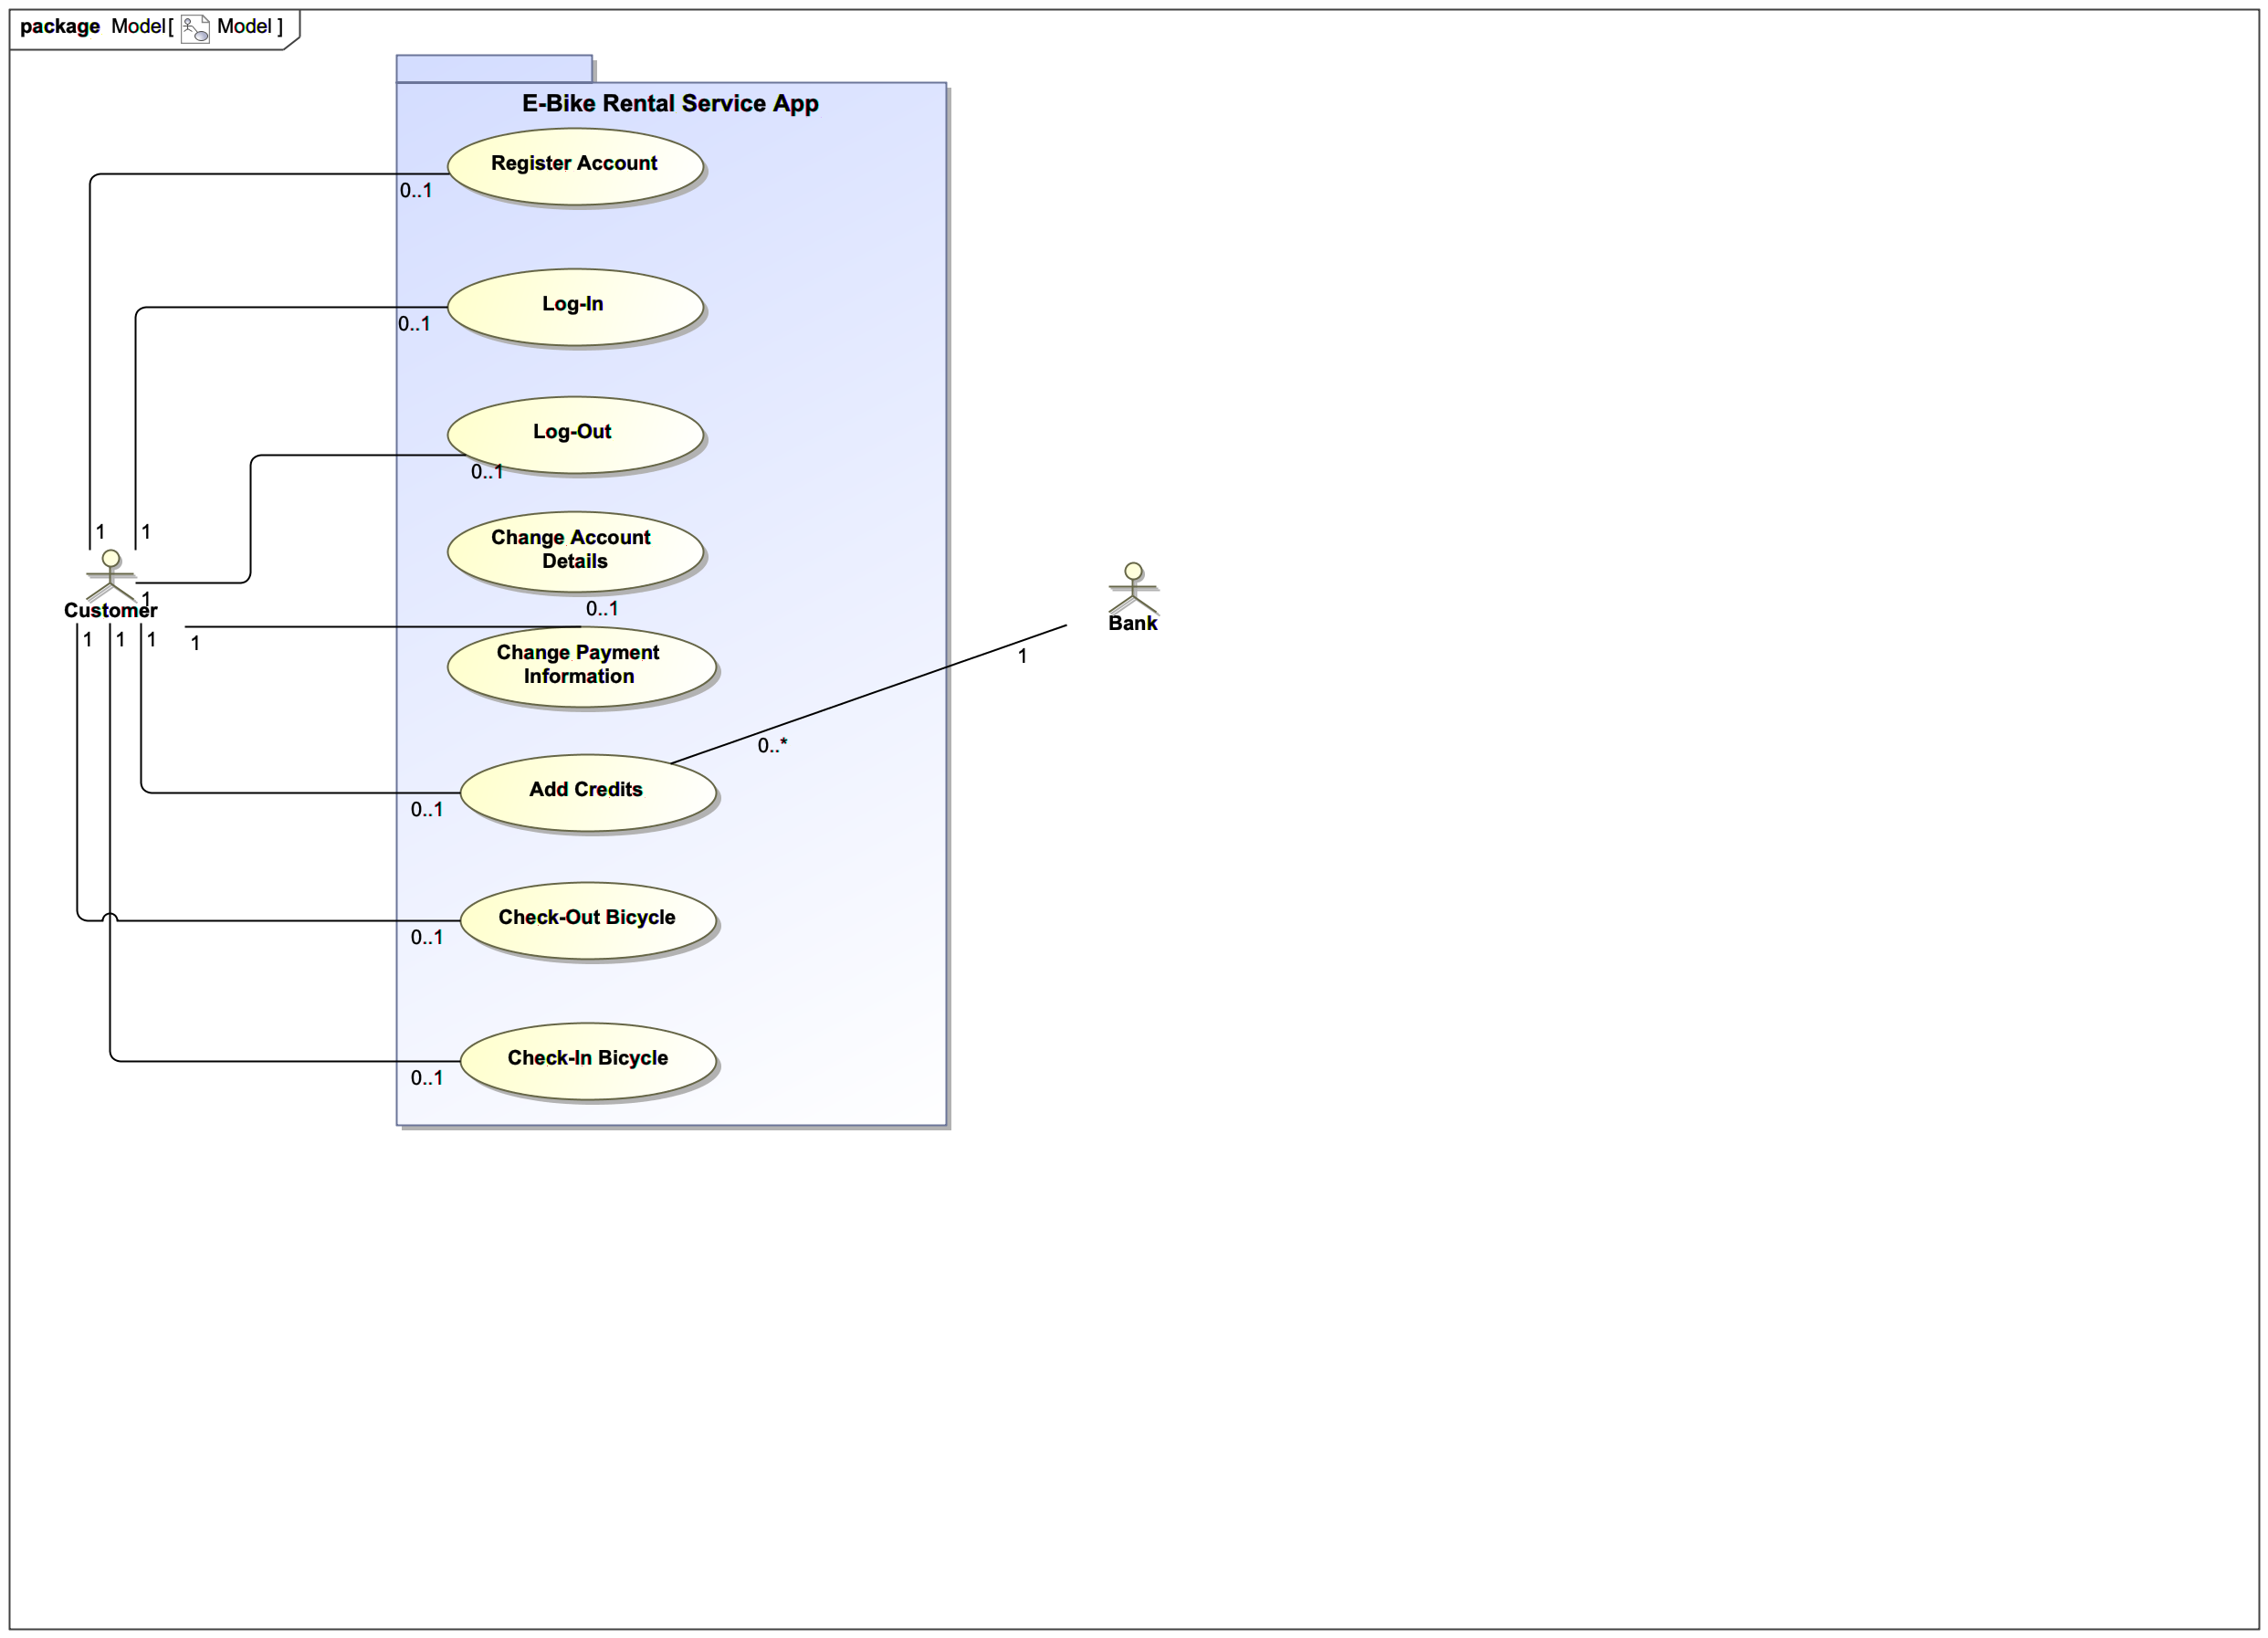
\includegraphics[scale=0.5]{02-e-bike-rental-service-variant-2.png}
\end{center}

\newpage
\section{Division of Work}
\renewcommand{\arraystretch}{1.5}
\begin{tabular}{|c|c|c|c|c|}
\hline
Kendra Birringer    & Nader Cacace  & Steffen Hanzlik   & Marco Peluso  & Svetozar Stojanovic\\
\hline
25\%                & 25\%          & 25\%              & 25\%          & 25\%\\
\hline
\end{tabular}
\newpage

\begin{thebibliography}{2}

\bibitem{uml251specpdf}
UML Standard 2.5.1 Specification\\
https://www.omg.org/spec/UML/2.5.1/PDF

\end{thebibliography}

\end{document}
